In this section, we have explored all the provided datasets to understand their properties, size and scale. We have also performed an analysis of how these datasets correlate with the provided problem.

\subsubsection{What are the different properties, size and scale of data?}

After importing all the provided datasets using \texttt{pandas} python package, we deduced following summary of the data as shown in the below tables.

\begin{table}[H]
\centering
\begin{tabular}{|l|l|l|}
\hline
\# & \textbf{Dataset Name} & \textbf{Dataset Description}                                           \\ \hline
1  & \texttt{uom-space}             &  7 campuses, 331 buildings, 28 floor codes, 5703 rooms, 185 room types             \\ \hline
2  & \texttt{rm-category-type}      & 209 different room types               \\ \hline
3  & \texttt{fl-name}               & floor information of all possible floor codes              \\ \hline
4  & \texttt{av-equipment}         & 1964 equipments, 32 manufacturers in 11 campuses across 142 buildings        \\ \hline
5  & \texttt{em-location}           & 7709 employees across 130 buildings and 1565 room codes                       \\ \hline
6  & \texttt{2020-timetable-v2}     & 52 departments, 1577 modules across 248 activity dates \\ \hline
7  & \texttt{meeting-room-usage}    & 890 meeting rooms across 8 campuses, 125 buildings                                   \\ \hline
\end{tabular}
\caption{Important categorical variables data summary}
\end{table}

\begin{table}[H]
\centering
\begin{tabular}{|l|l|l|}
\hline
\# & \textbf{Dataset Name} & \textbf{Dataset Description}                                           \\ \hline
1  & \texttt{uom-space}             &  Room Capacity: 0-599 with an $\mu$ of 4.0627 and $\sigma$ of 17.2592             \\ \hline
2  & \texttt{uom-space}             &  Room Area $m^2$: 0.22-5696.90 with an $\mu$ of 30.70 and $\sigma$ of 118.3070               \\ \hline                    
3  & \texttt{2020-timetable-v2}     & Planned Size: 0-684 with average of 50 students \\ \hline
4  & \texttt{2020-timetable-v2}     & Class Duration(min): 30-675 with an average of 94.336 \\ \hline
5  & \texttt{meeting-room-usage}    & Meetings: 0-1000 with an average of 241 meetings                                   \\ \hline
\end{tabular}
\caption{Important numerical variables data summary}
\end{table}

\subsubsection{How is the data distributed across problem statement?}

In our analysis, we explored different categorical and numerical features of the datasets to get more depth about the data. Initially, we saw that most of the data is provided for the \texttt{Parkville} campus as shown in Figure \ref{fig:expo-image-1}. Due to this huge skewness, we have performed our data and correlation analysis on the Parkville campus in this report, which can be easily extended to other campuses in the future phase of this project.

\begin{figure}[H]
\centering
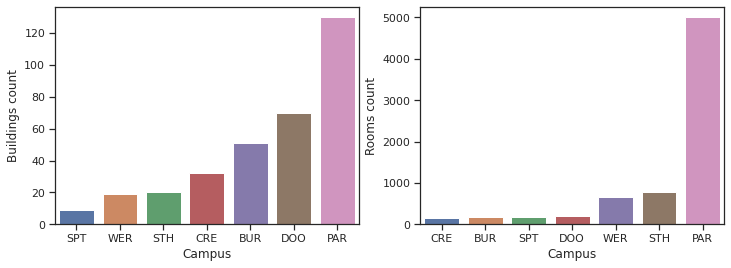
\includegraphics[width=12cm,keepaspectratio=true]{snap-1}
\caption{Distribution of buildings and rooms across campus}
\label{fig:expo-image-1}
\end{figure}

Using room category data and merging it with space metadata, we were able to figure out the distribution of meeting rooms and toilet facilities across buildings in the Parkville campus as shown in Figure \ref{fig:expo-image-2}. We saw that \texttt{333 Exhibition st} buildings have the highest number of meeting rooms and \texttt{The spot} building has the highest number of toilet facilities.

\begin{figure}[H]
\centering
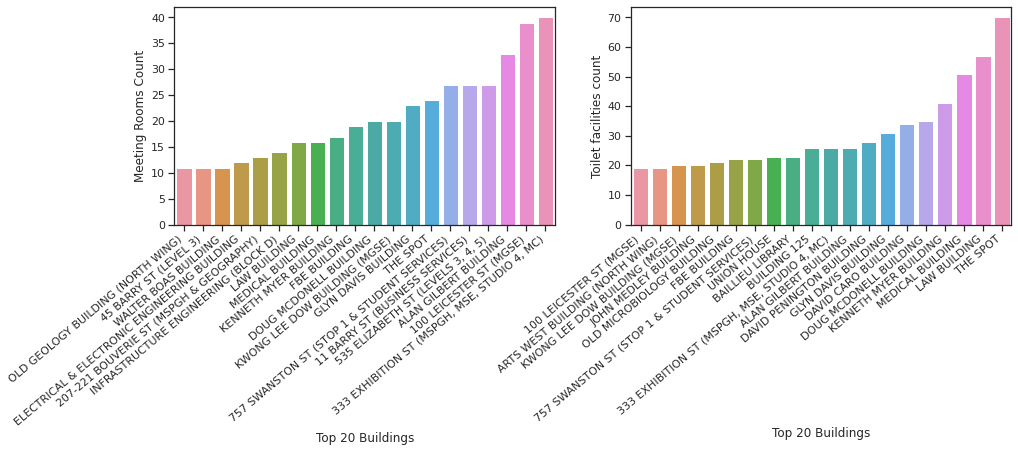
\includegraphics[width=16cm,keepaspectratio=true]{snap-2}
\caption{Distribution of meeting rooms and toilet facilities across buildings}
\label{fig:expo-image-2}
\end{figure}

% We did the same analysis on the employee data for the Parkville campus and saw that most of the staff members are located in \texttt{Doug Mcdonell Building} followed by \texttt{Business Services} building. They usually sit in the room which has \texttt{shared prostaff} or \texttt{shared grades} as their room types. Moreover, they are mostly located on the \texttt{Level 3} across buildings and mostly belong to the department \texttt{4140}.

% Similarly, analysis of audio-visual equipment dataset reveals that most of the equipment is of \texttt{Fuji Xerox} manufacturer with \texttt{Print staff} as their equipment standard. Most of the meeting rooms with equipment are found in \texttt{Kwong Lee Dow building} and they are usually located on \texttt{Level 1} across buildings.

% Finally, we did the same analysis on the timetable data and meeting room usage data. We saw that most of the classes are scheduled for \texttt{MDHS} department where \texttt{MGSE} department has the highest number of modules. Similarly, we saw that most of the meetings are being held at \texttt{Stop 1} building followed by \texttt{Alan gilbert} building where 84\% of these rooms are in \texttt{Excellent} condition.

\subsubsection{How is the data connected with the problem?}

After exploring different properties and aspects of the data, we tried to see and understand how data can be used to get the basic intuition of the problem.

To do that, we created several supply-demand plots across various covariates which helped to see the need for space optimization. Initially, we created supply-demand plots based on the very trivial preference of staff members trying to book a meeting room in the same building where they are located. This plot is shown in Figure \ref{fig:expo-image-3}. As per the plot, we can see space optimization problem in terms of supply and demand proportion especially in the \texttt{Law Building}, \texttt{Doug Mcdonell building} and \texttt{Kenneth Myer building}.

\begin{figure}[H]
\centering
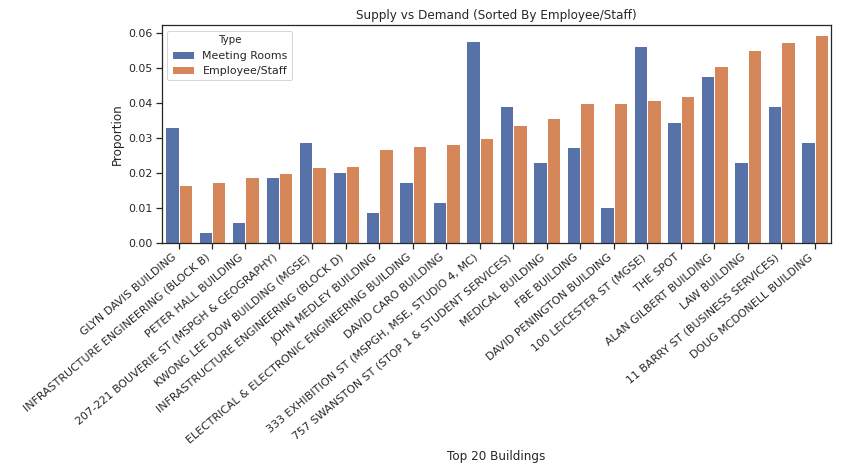
\includegraphics[width=10cm,keepaspectratio=true]{snap-3}
\caption{Supply vs Demand of meeting rooms across buildings}
\label{fig:expo-image-3}
\end{figure}

 Similarly, we created a supply-demand plot on the same trivial preference of students trying to access a toilet facility in the same building which is shown in Figure \ref{fig:expo-image-4}. Again, we can see that the space optimization problem in terms of supply and demand proportion, especially for \texttt{Redmond barry building}.
 
\begin{figure}[H]
\centering
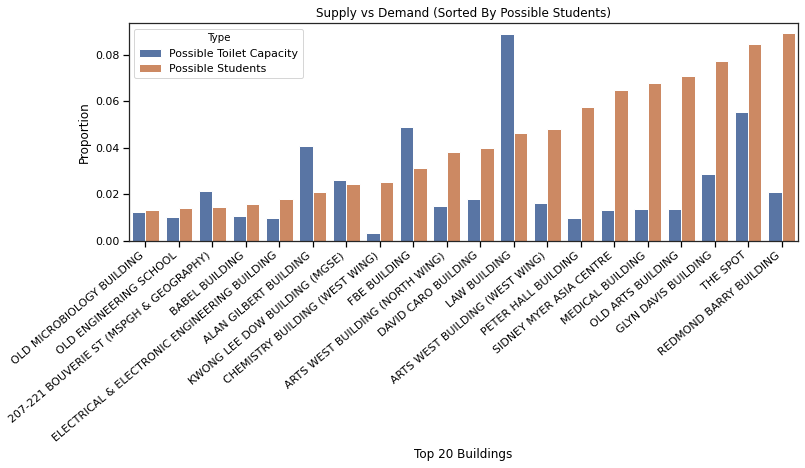
\includegraphics[width=10cm,keepaspectratio=true]{snap-4}
\caption{Supply vs Demand of toilet facilities across buildings}
\label{fig:expo-image-4}
\end{figure}

We have explored several other covariates concerning supply-demand in Section \ref{correlations} which will eventually help us to perform space optimization on the underlying problem.